\subtitlepage{SaltStack}{Эксплуатация}

\begin{Frame}{Команды}

  \overlaypic{south east}{width=80pt}{terminal}

  \begin{itemize}[<+-| alert@ +>]
    \item \texttt{salt-key} \ExampleIcon{}
    \vfill
    \item \texttt{salt ЦЕЛЬ МОДУЛЬ.ФУНКЦИЯ АРГУМЕНТЫ}
    \vfill
    \item \texttt{salt-cp ЦЕЛЬ ИСТОЧНИК1 [ИСТОЧНИК2 \dots] НАЗНАЧЕНИЕ}
    \vfill
    \item \texttt{salt-call МОДУЛЬ.ФУНКЦИЯ АРГУМЕНТЫ}
    \vfill
    \item \texttt{salt-run МОДУЛЬ.ФУНКЦИЯ АРГУМЕНТЫ}
  \end{itemize}
\end{Frame}

\begin{Frame}{Нацеливание}
  \ExampleNote{}

  \begin{itemize}[<+-| alert@ +>]
    \item[\faBullseye] По имени\footnote<.->{Помним, что * без кавычек
      раскрывается шеллом}\\
      \footnotesize \texttt{salt '*-blue' test.ping}
    \item[\faBullseye] По грейнам\\
      \footnotesize \texttt{salt -G 'os:CentOS Stream' test.ping}
    \item[\faBullseye] По группам\\
      \footnotesize \texttt{salt -N blue test.ping}
    \item[] \ldots
    \item[\faBomb] Комбинируя условия почти как угодно\footnote{Разбивка по
    пробелам, пробелы напрямую передать не получится
    (\uhref{https://github.com/saltstack/salt/issues/21260}{\#21260})}\\
      \footnotesize
      \texttt{salt -C '( G@os:CentOS* and *blue ) or S@192.168.122.112'
      test.ping}
  \end{itemize}
\end{Frame}

\begin{Frame}{Шина событий}

  \begin{itemize}[<+-| alert@ +>]
    \item[{\faComments[regular]}] Это как общий чат
    \item[{\faBell[regular]}] Авторизованные клиенты подписываются
    \item[{\faHandPaper[regular]}] Миньоны берут задачи, когда они есть в адресатах
    \item[{\faCommentDots[regular]}] Миньоны отвечают обратно в шину
    \item[\faFighterJet] Шина на ZeroMQ производительна
    \item[\faTerminal] \texttt{salt-run state.event [ПАТТЕРН\_СОБЫТИЯ]
      [pretty=True]}
  \end{itemize}

\end{Frame}

\begin{Frame}{Модули исполнения}
  \ExampleNote{}

  \begin{itemize}[<+-| alert@ +>]
    \item \texttt{test, saltutil}
    \item \texttt{file, pkg, service, system, cmd\dots}
    \item \texttt{apache, postgres, nginx, redis\dots}
    \item \texttt{ansiblegate, chef, puppet}
  \end{itemize}
\end{Frame}

\begin{Frame}{Пара полезных функций}

  \overlaypic{south east}{width=80pt}{note}

  \begin{itemize}[<+-| alert@ +>]
    \setbeamertemplate{itemize item}{\faTerminal}
    \item \texttt{test.ping}\vfill
    \item \texttt{saltutil.sync\_all}\vfill
    \item \texttt{sys.doc}\vfill
    \item \texttt{state.test}\footnote{добавлена в 3001 как алиас для
      \texttt{state.apply test=True}}\vfill
  \end{itemize}
  \vfill

\end{Frame}

\begin{Frame}{Формулы}

  \framesubtitle{Основные свойства}

  \begin{columns}
    \begin{column}{0.6\textwidth}
      \begin{itemize}[<+-| alert@ +>]
        \item[\faBook] Местные cookbook'и
        \baselinespace{}
        \item[\faRedo] Идемпотентность (повторяемость)
        \baselinespace{}
        \item[\faRocket] Топ-файл и хайстейт \ExampleIcon{}
      \end{itemize}
    \end{column}

    \begin{column}{0.4\textwidth}
      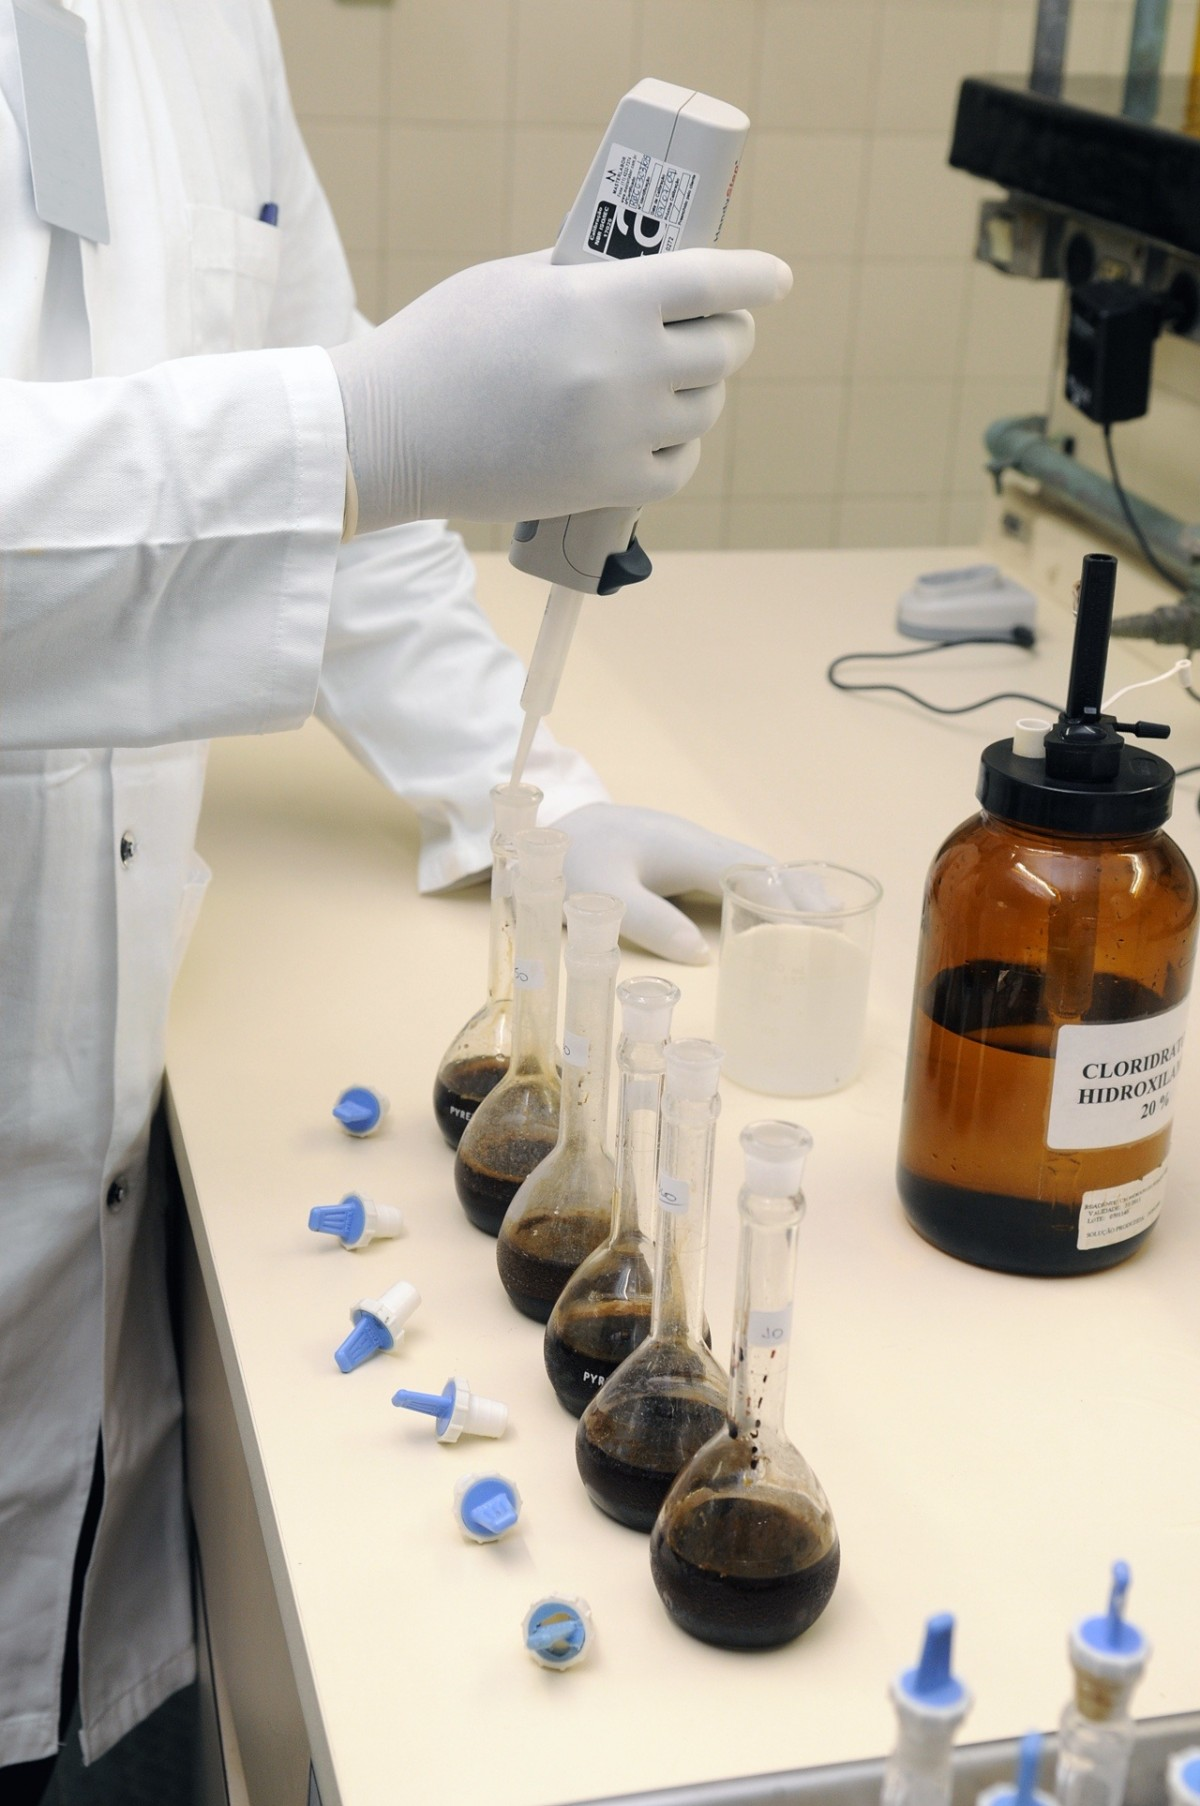
\includegraphics[height=0.75\textheight]{chemist}
    \end{column}
  \end{columns}

\end{Frame}

\begin{frame}[fragile]{Формулы}
  \framesubtitle{Синтаксис}

  \begin{columns}
    \begin{column}{0.25\textwidth}
      \begin{minted}[gobble=8]{salt}
        my_state_id1:
          states_module1.function1
          states_module2.function2:
            - name: overrided_id
            - arg1: value
            - arg2:
                - value1
                - value2
                - value3

        my_state_id2:
          states_module1.function1
      \end{minted}
    \end{column}
    \begin{column}{0.65\textwidth}
      \onslide<+->
      \begin{itemize}[<+-| alert@ +>]
        \footnotesize
        \item Функции состояний принимают аргумент \texttt{name}
        \baselinespace{}
        \item \texttt{name} по умолчанию равен идентификатору
        \baselinespace{}
        \item В формуле может быть множество состояний
        \baselinespace{}
        \item В состоянии можно обращаться к нескольким разным модулям
        \baselinespace{}
        \item В состоянии нельзя обращаться к одному модулю несколько раз
      \end{itemize}
    \end{column}
  \end{columns}
\end{frame}

\begin{frame}{Формулы}
  \framesubtitle{Синтаксис}
  \centering
  \Large
  \inlineicon{\faBomb}Часто можно сделать одно разными путями\\
  \baselinespace{}
  \pause{}
  \inlineicon{\faLightbulb} Хорошо выбрать один способ и придерживаться его
\end{frame}

\begin{Frame}{Модули состояния}
  \begin{itemize}[<+-| alert@ +>]
    \item \texttt{test, saltutil}
    \item \texttt{file, pkg, service, system, \bfseries{cmd}\dots}
    \item \texttt{apache, postgres\_*, redismod\dots}
    \item \texttt{ansiblegate, chef}
  \end{itemize}

  \vfill

  \centering
  \onslide<+->
  Всего на сегодня 349 штук согласно документации
  \only<.>{\overlaypic{south east}{width=100pt}{peaks}}
\end{Frame}

\liveframe{}

\begin{Frame}{Порядок разбора}
  \begin{enumerate}[<+-| alert@ +>]
    \item[0] Разбор на миньоне
    \baselinespace{}
    \item Рендеринг (\texttt{jinja | yaml})
    \baselinespace{}
    \item Определение порядка исполнения
    \baselinespace{}
    \item Исполнение
  \end{enumerate}
  \baselinespace{}

  \centering

  \onslide<+->
  \inlineicon{\faExclamationTriangle} При ошибке на любом этапе --- ответ в шину
\end{Frame}

\begin{Frame}{Порядок исполнения}
  \framesubtitle{Варианты}

  Три пути:
  \vfill
  \begin{enumerate}[<+-| alert@ +>]
    \item В лексикографическом порядке \ExampleIcon{}
    \vfill
    \item По флагу \texttt{order} \ExampleIcon{}
    \vfill
    \item По реквизитам \ExampleIcon{}
  \end{enumerate}

  \centering
  \vfill
  \onslide<+->
  \inlineicon{\faStickyNote} Документация призывает выбрать один способ, и
  следовать ему

  \vfill
\end{Frame}

\begin{frame}{Порядок исполнения}
  \framesubtitle{Предупреждение}
  \begin{center}
    
\includegraphics[height=0.6\textheight]{mess}\\
    \inlineicon{\faRecycle} Реквизиты позволяют элегантно запутать ваш код
      \inlineicon{\faBug}
  \end{center}
\end{frame}

\liveframe{}

\Setsubsection{Каверзы YAML}
\begin{frame}[fragile]
  \frametitle{\Insertsubsection}

  \begin{itemize}[<+-| alert@ +>]
    \item[{\faFrown[regular]}] Стандарт регламентирует использование пробелов
    \item[{\faCheckCircle[regular]}] Не используйте табы

    \vfill

    \item[{\faFrown[regular]}] Вложенный словарь проигнорирован
    \item[{\faCheckCircle[regular]}] Увеличивать отступ
  \end{itemize}

  \vfill

  \begin{columns}
    \begin{column}{0.3\textwidth}
     \onslide<3->
      \begin{minted}[gobble=8]{yaml}
        tree:
          - branch1:
            leaf1: yellow
            leaf2: green
          - branch2:
            leaf1: yellow
      \end{minted}
    \end{column}

    \begin{column}{0.3\textwidth}
      \onslide<4->
      \begin{minted}[gobble=8]{yaml}
        tree:
          - branch:
              leaf1: yellow
              leaf2: green
          - branch:
              leaf1: yellow
      \end{minted}
    \end{column}
  \end{columns}

\end{frame}

\begin{frame}{Каверзы YAML}
  \begin{itemize}[<+-| alert@ +>]
    \item[{\faFrown[regular]}] \texttt{Yes, yes, No, no} и т.~д. грузятся
      как буль
    \item[{\faCheckCircle[regular]}] Оборачивать кавычками

    \vfill

    \item[{\faFrown[regular]}] По стандарту только ASCII
    \item[{\faCheckCircle[regular]}] Стараться использовать ASCII, не вставлять emoji
      \faSmile[regular]
  \end{itemize}
\end{frame}

\begin{frame}{Каверзы YAML}
  \begin{itemize}[<+-| alert@ +>]
    \item[{\faFrown[regular]}] Строки с датой приводятся к \texttt{datetime}, а с
      временем --- к целым
    \item[{\faCheckCircle[regular]}] Оборачивать кавычками

    \vfill

    \item[{\faFrown[regular]}] Символ \texttt{\%} имеет специальное значение, символ
      \texttt{\_} игнорируется в целочисленных литералах
    \item[{\faCheckCircle[regular]}] Кавычки
  \end{itemize}
\end{frame}

\begin{Frame}[c]{Полезные ссылки}
  \setbeamertemplate{itemize items}[square]
  \begin{itemize}
    \setbeamertemplate{itemize item}{\faLink}
    \item[\faBook]
      \uhref{https://docs.saltproject.io/en/latest/contents.html}{%
      Генерируемая документация} (можно скачать \faDownload)
    \item[\faGithub] Когда что-то не работает, наперёд шерст\'им
      \uhref{https://github.com/saltstack/salt/issues}{тикеты на GitHub}
  \end{itemize}
\end{Frame}
